\documentclass[a4paper,11pt]{article}
\pdfoutput=1 % if your are submitting a pdflatex (i.e. if you have
             % images in pdf, png or jpg format)

\usepackage{jheppub} % for details on the use of the package, please
                     % see the JHEP-author-manual
\usepackage{dsfont}
\usepackage[T1]{fontenc} % if needed
\usepackage{subcaption}
\usepackage{array}   % for \newcolumntype macro
\newcolumntype{L}{>{$}l<{$}} % math-mode version of "l" column type
\usepackage{caption}




\title{\boldmath Notes on bootstrapping the $O(N)$ vector models with a boundary}


%% %simple case: 2 authors, same institution
%% \author{A. Uthor}
%% \author{and A. Nother Author}
%% \affiliation{Institution,\\Address, Country}

% more complex case: 4 authors, 3 institutions, 2 footnotes
% \author[a,b,1]{F. Irst,\note{Corresponding author.}}
% \author[c]{S. Econd,}
% \author[a,2]{T. Hird\note{Also at Some University.}}
% \author[a,2]{and Fourth}
\author[a]{Jaychandran Padayasi}

% The "\note" macro will give a warning: "Ignoring empty anchor..."
% you can safely ignore it.

\affiliation[a]{The Ohio State University,\\Columbus, OH, USA}
% \affiliation[b]{Another University,\\different-address, Country}
% \affiliation[c]{A School for Advanced Studies,\\some-location, Country}

% e-mail addresses: one for each author, in the same order as the authors
\emailAdd{padayasi.1@osu.edu}
% \emailAdd{second@asas.edu}
% \emailAdd{third@one.univ}
% \emailAdd{fourth@one.univ}




\abstract{Abstract...}



\begin{document} 
\maketitle
\flushbottom

\section{Introduction}
\label{sec:intro}

The nature of the boundary universality classes in the $O(N)$ models in $d = 3$ dimensions is an interesting problem which has not yet been settled in the literature of statistical mechanics. Recently, using innovative methods in the renormalization group, \cite{Max} was able to show that the models could afford a slew of interesting features as a function of $N$. Key results from \cite{Max} were that the special fixed point exists for $N = 2$ and also for $N \rightarrow 2^+$ but it separates the ordinary transition from an "extra-ordinary log" transition. Upon increasing $N$, eventually the special FP moves and fuses into the ordinary FP at some critical value $N_c$ (not necessarily an integer). If $N_c > 3$, these phases could be realized in experiments. In the approach of \cite{Max}, $N_c$ depends on certain universal constants related to the normal fixed point (which exists for all $N$ in $d = 3$). These constants are accessible by conformal bootstrap, and in these notes we outline our efforts in calculating them from known methods of the boundary bootstrap program. 

\subsection{Conformal bootstrap in the presence of a boundary}
\label{sec:CBB}
The idea of conformal bootstrap is quite old, dating back to Polyakov \cite{Polyakov} but it has gained traction since 2010 with the advent of powerful methods which work generally and have also been matched by the computational power required to solve the bootstrap equations. The boundary bootstrap was described in the same spirit as this revival in \cite{Liendo} using some mathematical results from \cite{Mcavity}. In this section, we recall important results from these works, especially about the boundary conformal blocks.

Consider a $d$-dimensional CFT with a codimension-1 boundary (say, at $x^d = 0$). In this case, the full conformal symmetry of the theory is broken down to a subgroup that leaves $x^d = 0$ invariant. Under this subgroup, one can construct the invariant cross ration $\xi$,
\begin{equation}
    \xi = \frac{(\textbf{x} - \textbf{y})^2}{4x^dy^d}
\end{equation}
The existence of an invariant quantity composed of two points $x = (\textbf{x}, x^d)$ and $y = (\textbf{y}, y^d)$ implies the existence of an arbitrary function of $\xi$ in the two-point functions. Conformal blocks are decompositions of $n$-point functions in terms of the operator product expansion (OPE) of the CFT. For bulk CFTs, non-trivial conformal blocks occur only for 4-point functions. However, in the presence of a boundary, due to the coupling between the surface and the bulk operators, even 2-point functions could have non-trivial conformal block expansions. 

Consider the (bulk) OPE involving two identical scalars
\begin{equation}
    \mathcal{O}\times\mathcal{O} \sim \sum_k\mathcal{O}_k
\end{equation}

We will assume that the one-point functions of operators are, in general, not zero. Instead, they are given by the identity contribution of the boundary OPE. This is because, the operators that live on the boundary, $\hat{\mathcal{O}}_l$ form a valid basis for representing the 2-point functions. Thus, we have
\begin{equation}
    \mathcal{O}_k \sim \hat{\mathds{1}} + \sum_l \hat{\mathcal{O}}_l
\end{equation}
where $\hat{\mathcal{O}}_l$ belong to the $SO(d,1)$ CFT that exists at the boundary $x^d = 0$. As the one-point function of the identity in any CFT is non-zero,

\begin{equation}
\label{eq:BOPE}
    \langle \mathcal{O}_k(x) \rangle = \frac{a_k}{(2x^d)^{\Delta_k}}
\end{equation}
where $a_k$ is an OPE coefficient between the bulk operator and the boundary identity. 

Using these OPEs, we can find the behavior of 2-point functions of bulk operators in different limits. Consider the bulk limit, $\xi \rightarrow 0$ or $\textbf{x} - \textbf{y} \ll x^d, y^d$,
\begin{align}
    \langle \mathcal{O}(x)\mathcal{O}(y)\rangle &= \sum_k \frac{\lambda_{k}\left\langle\mathcal{O}_k\left(\frac{x + y}{2}\right)\right\rangle}{(\textbf{x} - \textbf{y})^{2\left(\Delta_{\mathcal{O}} - \Delta_k/2\right)}}\Tilde{f}_{\textrm{bulk}}(\Delta_k, x, y) \\
    &= \sum_k \frac{a_k\lambda_{k}}{(\textbf{x} - \textbf{y})^{2\Delta_{\mathcal{O}}}}\xi^{\Delta_k/2}\Tilde{f}_{\textrm{bulk}}(\Delta_k, x, y) \equiv \sum_k a_k\lambda_kf_{\textrm{bulk}}(\Delta_k, \xi)
\end{align}
where $\lambda_k$ are bulk OPE coefficients. In the boundary limit ($\xi \rightarrow \infty$), each operator is expanded in the basis of boundary operators \textit{first}, and then two-point functions are calculated in the boundary CFT. Here, we must use a different conformal block $f_{\textrm{bdy}}$:
\begin{equation}
    \langle \mathcal{O}(x)\mathcal{O}(y)\rangle = \sum_k \frac{\mu_{\mathcal{O}k}^2\langle\hat{\mathcal{O}}_k(\textbf{x})\hat{\mathcal{O}}_k(\textbf{y})\rangle}{(4x^dy^d)^{(\Delta_{\mathcal{O}} - \Delta_{\hat{k}})}}\Tilde{f}_{\textrm{bdy}}(\Delta_{\hat{k}}, x, y)
\end{equation}
where $\mu_{\mathcal{O}k}$ is an OPE coefficient of \ref{eq:BOPE} and $\Delta_{\hat{k}}$ is the corresponding scaling dimension of the boundary operator. Using
\begin{equation}
    \langle\hat{\mathcal{O}}_k(\textbf{x})\hat{\mathcal{O}}_k(\textbf{y})\rangle = \frac{1}{(\textbf{x} - \textbf{y})^{2\Delta_{\hat{k}}}},
\end{equation}
the 2-point function takes the form
\begin{equation}
    \langle \mathcal{O}(x)\mathcal{O}(y) \rangle =  \sum_k \frac{\mu_{\mathcal{O}k}^2}{(4x^dy^d)^{\Delta_{\mathcal{O}}}}\xi^{-\Delta_{\hat{k}}}\Tilde{f}_{\textrm{bdy}}(\Delta_{\hat{k}}, x, y) \equiv \sum_k \mu_{\mathcal{O}k}^2f_{\textrm{bdy}}(\Delta_{\hat{k}}, \xi)
\end{equation}
As explained in the Appendix A of \cite{Liendo}, these leading behaviors are enough to derive the functions $f_{\textrm{bulk}}$ and $f_{\textrm{bdy}}$ from the Casimirs of $SO(d+1, 1)$ and $SO(d,1)$ respectively. 

\section{Deriving the bootstrap equations}

In this section, we write the relevant OPEs and derive the crossing equations therefrom. We will be working around the normal fixed point, so the boundary is forced to order along, say, the $1$-axis. Thus, it is important to consider the longitudinal component separately from the transverse ones. Following \cite{Max}, we call these $\sigma$ and $\phi_i$ respectively, with $i$ running from 2 to $N$. As is common in boundary bootstrap literature \cite{Liendo}\cite{Gliozzi}, we will denote operators living on the boundary with a hat $(\hat{\sigma}, \hat{\phi})$. We will be considering the following two-point function:
\begin{equation}
\label{eq:Corr}
    \langle \sigma(\textbf{x},x^d)\sigma(\textbf{y}, y^d) \rangle + \left\langle \sum_{i = 2}^N \phi_i(\textbf{x}, x^d) \phi_i(\textbf{y}, y^d) \right\rangle
\end{equation} 
for which we need to write down the OPEs of the fields in the bulk and boundary channels. Note that in each correlator in \ref{eq:Corr}, the boundary identity is implied (e.g. $\langle\sigma\sigma\hat{\mathds{1}}\rangle$). In the bulk channel, both $\sigma$ and $\phi_i$ should have the same OPEs, as we expect $O(N)$ symmetry to be preserved in that limit. Thus, they are characterised by the same CFT data (scaling dimensions and OPE coefficients). The allowed terms in the OPE are dictated by the representation theory of $O(N)$ \cite{Kos}:
\begin{equation}
    \phi_i \times \phi_j \sim \sum_{S^+} \delta_{ij}\mathcal{O} + \sum_{T^+}\mathcal{O}_{(ij)} + \sum_{A^-}\mathcal{O}_{[ij]}
\end{equation}
where $S$, $T$ and $A$ denote $O(N)$ singlets, symmetric traceless tensors and anti-symmetric tensors respectively. The effect of considering the two-point function \ref{eq:Corr} is to eliminate the last two terms in the bulk-channel OPE. Thus we only deal with $O(N)$ singlets in the bulk channel. 

In the boundary channel, the longitudinal component $\sigma$ must couple to the boundary identity, so that it acquires a non-zero expectation value. We also know that the next leading operator for the longitudinal component must be the displacement operator $\hat{D}$ with dimension $\Delta_{\hat{D}} = d = 3$ associated with the breaking of translation invariance along the $d$-axis. Thus, we have
\begin{subequations}
\begin{equation}
    \sigma \sim \hat{\mathds{1}} + \hat{D} + \ldots
\end{equation}
\begin{equation}
    \phi_i \sim \hat{\phi_i} + \ldots
\end{equation}
\end{subequations}
where $\hat{\phi_i}$ has scaling dimension $d - 1$. Using these operator product expansions, the two-point function can be written in terms of the boundary conformal blocks (~\cite{Mcavity}). In the bulk channel, we have
\begin{equation}
    \langle\sigma\sigma\rangle + \sum_{i = 2}^N\langle\phi_i\phi_i\rangle = \frac{N}{(x-y)^{2\Delta_{\phi}}} + \sum_k N\lambda_{\phi\phi k}a_k\Tilde{f}_{\text{bulk}}(\Delta_k, x, y),
\end{equation}
where the sum runs over relevant $\mathcal{O}(N)$ singlet, Lorentz scalar operators. $\Delta_{\phi} = \frac{1 + \eta}{2}$ is a known exponent whereas all OPE coefficients are to be treated as unknowns. In the boundary channel, 
\begin{multline}
  \langle\sigma\sigma\rangle + \sum_{i = 2}^N\langle\phi_i\phi_i\rangle = \frac{a_{\sigma}^2}{(2x^d)^{\Delta_{\phi}}(2y^d)^{\Delta_{\phi}}} + \mu_{\sigma D}^2\Tilde{f}_{\text{bdy}}(d;\textbf{x}, \textbf{y})\\ + (N-1)\mu_{\phi\phi}^2\Tilde{f}_{\text{bdy}}(d-1;\textbf{x}, \textbf{y}) + \ldots 
\end{multline}
The functions $\Tilde{f}_{\text{bulk}}$ and $\Tilde{f}_{\text{bdy}}$ can be expressed in terms of the invariant cross ratio $\xi(x, y)$ as hypergeometric functions upto an overall scale factor \cite{Mcavity}\cite{Liendo}. Following the discussion in Section \ref{sec:CBB},
\begin{subequations}
\begin{equation}
    f_{\text{bulk}}(\Delta, \xi) = \xi^{\Delta/2} \ _2F_1\left(\frac{\Delta}{2}, \frac{\Delta}{2};\Delta + 1 - \frac{d}{2}, -\xi\right) \equiv (x-y)^{2\Delta_{\phi}}\Tilde{f}_{\text{bulk}},
\end{equation}
\begin{equation}
    f_{\text{bdy}}(\Delta, \xi) = \xi^{-\Delta}\ _2F_1\left(\Delta, \Delta + 1 - \frac{d}{2}; 2\Delta + 2 - d; -\frac{1}{\xi}\right) \equiv (4x^dy^d)^{\Delta_{\phi}}\Tilde{f}_{\text{bdy}}.
\end{equation}
\end{subequations}
With these definitions, we can express crossing symmetry in the bulk and boundary channels as
\begin{equation}
\label{eq:Cross}
    N + \sum_k N\lambda_{\phi\phi k}a_kf_{\text{bulk}}(\Delta_k, \xi) = \xi^{\Delta_{\phi}}\left(a_{\sigma}^2 + (N-1)\mu_{\phi\phi}^2f_{\text{bdy}}(d-1,\xi) + \mu_{\sigma D}^2f_{\text{bdy}}(d, \xi)\right)
\end{equation}
up to the order in the boundary operators that we have defined in the OPE. This crossing equation is amenable to be solved self-consistently for the unknown CFT data by Gliozzi's truncation method (\cite{Gliozzi}).

The gist of the truncation method is that certain OPE's are `truncable', so that we can only keep the low-lying operators in the spectrum. Then, the crossing equation \ref{eq:Cross} can be expanded around some cross-ratio value, say $\xi = 1$. This way, we obtain infinitely many homogeneous equations involving the derivatives of conformal blocks evaluated at $\xi = 1$, of which we can keep the first $M$. 
The inhomogeneous equation becomes
\begin{equation}
-\left(\sum_{k = 1}^{n_{\text{bulk}}} N p_kf_{\text{bulk}}(\Delta_k, 1)\right) + a_{\sigma}^2 + (N - 1)\mu_{\phi\phi}^2f_{\text{bdy}}(d-1, 1) + \mu_{\sigma D}^2f_{\text{bdy}}(d,1) = N,
\end{equation}
where $p_k = \lambda_{\phi\phi k}a_k$. The homogeneous equations are,
\begin{multline}
   -\left(\sum_{k = 1}^{n_{\text{bulk}}} N p_k\left.\partial_m f_{\text{bulk}}(\Delta_k, \xi)\right|_{\xi = 1}\right) + (N - 1)\mu_{\phi\phi}^2\left.\partial_m(\xi^{\Delta_{\phi}}f_{\text{bdy}}(d-1, \xi))\right|_{\xi = 1}\\
        + \mu_{\sigma D}^2\left.\partial_m(\xi^{\Delta_{\phi}}f_{\text{bdy}}(d,\xi))\right|_{\xi = 1} + (\Delta_{\phi})_{m}\ a_{\sigma}^2 = 0
\end{multline}
for $m = 1,2,\ldots M$. This forms a homogeneous system of equations for the vector $(Np_k, (N-1)\mu_{\phi\phi}^2, \mu_{\sigma D}^2, a_{\sigma}^2 )$ of dimension $L = n_{\text{bulk}} + 3$ that is overconstrained if we choose $M > L$. It has a non-trivial solution only if the minimum singular value of the matrix of derivatives is zero \cite{Leclair}. Once the unknown dimensions are found, we can solve the system of homogeneous equations along with the inhomogeneous equation to obtain the OPE coefficients.

\section{Results for low integer $N$}
\label{sec:res}
In this section, we present our bootstrap results for integer values of $N$, up to $N = 4$. For $N = 1$, the analysis in \cite{Gliozzi} carries over, and our results corroborate excellently with the values in their work. The only difference in our methods is that we minimize the minimum singular value of the derivative matrix whereas \cite{Gliozzi} find the dimensions by requiring that all minors of order $L$ vanish. In the bulk channel, we kept four scalar operators apart from the identity. One of these is the energy (related to $\nu$ by $\Delta_{\epsilon} = 3 - 1/\nu$) and the next scalar operator is related to the exponent $\omega$ \cite{Gliozzi}. Bootstrap dictates the other two dimensions. Explicitly, we have the bulk OPE
\begin{equation}
    \phi_i \times \phi_i \sim \mathds{1} + \epsilon + \epsilon' + \epsilon'' + \epsilon'''
\end{equation}
with 
\begin{equation}
    \Delta_\phi = \frac{1 + \eta}{2}, \hspace{0.5in} \Delta_{\epsilon} = 3 - \frac{1}{\nu}, \hspace{0.5in} \Delta_{\epsilon'} = 3 + \omega.
\end{equation}
We use the critical exponents gathered in \cite{Gliozzi} and for $N = 4$, we take the results from \cite{Guida}.
For $N = 1$, we found a consistent solution at
\begin{equation}
    \Delta_{\epsilon''} = 7.34(84), \hspace{0.5 in}\Delta_{\epsilon'''} = 13.4(28)
\end{equation}
with the OPE coefficients
\begin{center}
\begin{tabular}{L L L}
    a_{\epsilon}\lambda_{\phi\phi\epsilon} = 6.909, &a_{\epsilon'}\lambda_{\phi\phi\epsilon} = 2.262, &a_{\epsilon''}\lambda_{\phi\phi\epsilon''} = 0.186, \\
    a_{\epsilon'''}\lambda_{\phi\phi\epsilon'''} = 0.003924,
    &a_{\sigma}^2 = 6.7537,
    &\mu_{\sigma D}^2 = 0.06285.
    
\end{tabular}  
\end{center}
\begin{figure}
% \captionsetup[subfigure]{justification=centering}

\begin{subfigure}{\columnwidth}
    \centering
    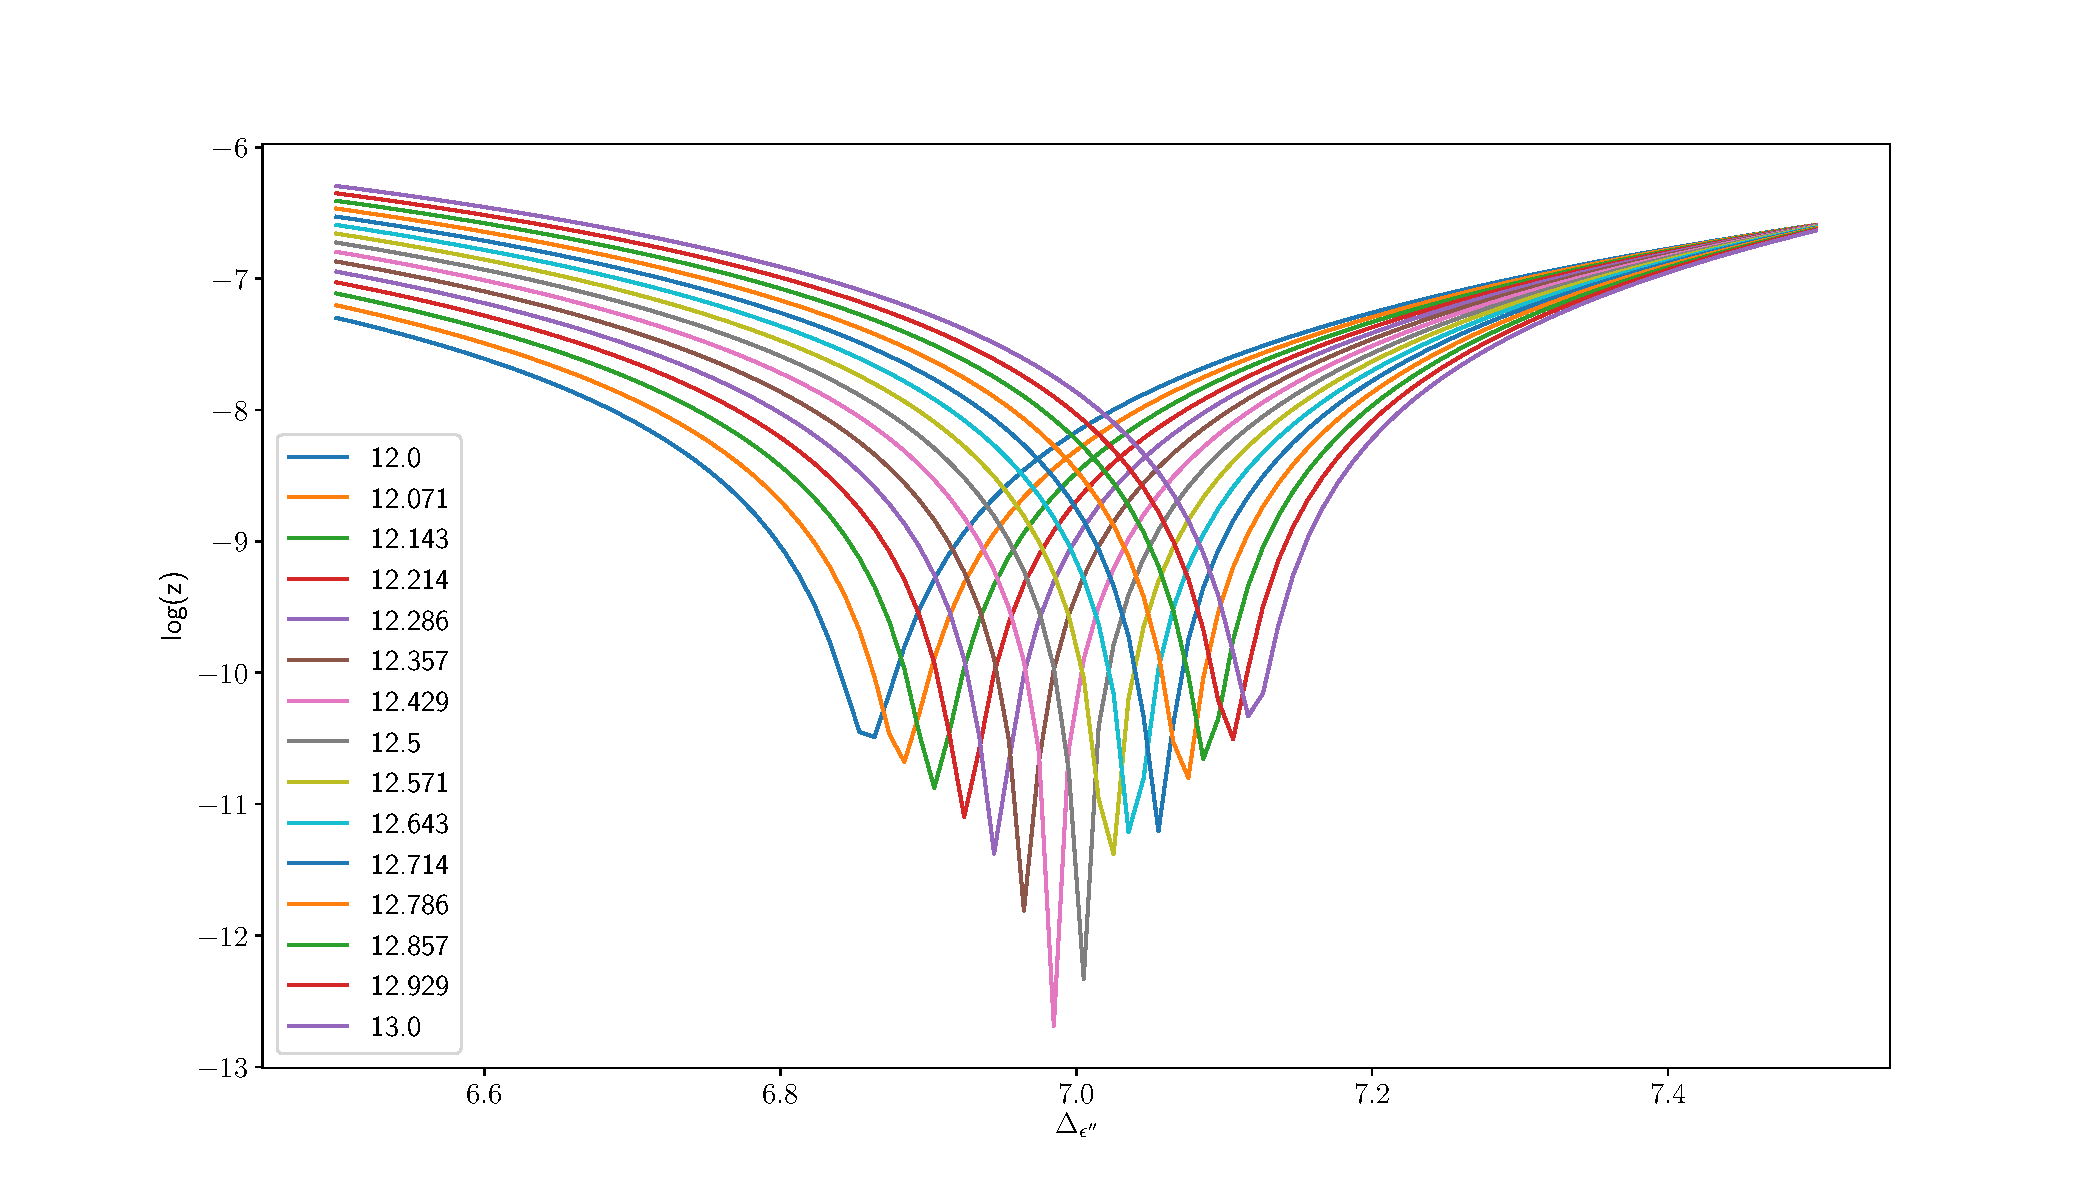
\includegraphics[scale=0.45]{Normal_N2.pdf}
    \caption{$N = 2$}
\end{subfigure}
~

\begin{subfigure}{\columnwidth}
    \centering
    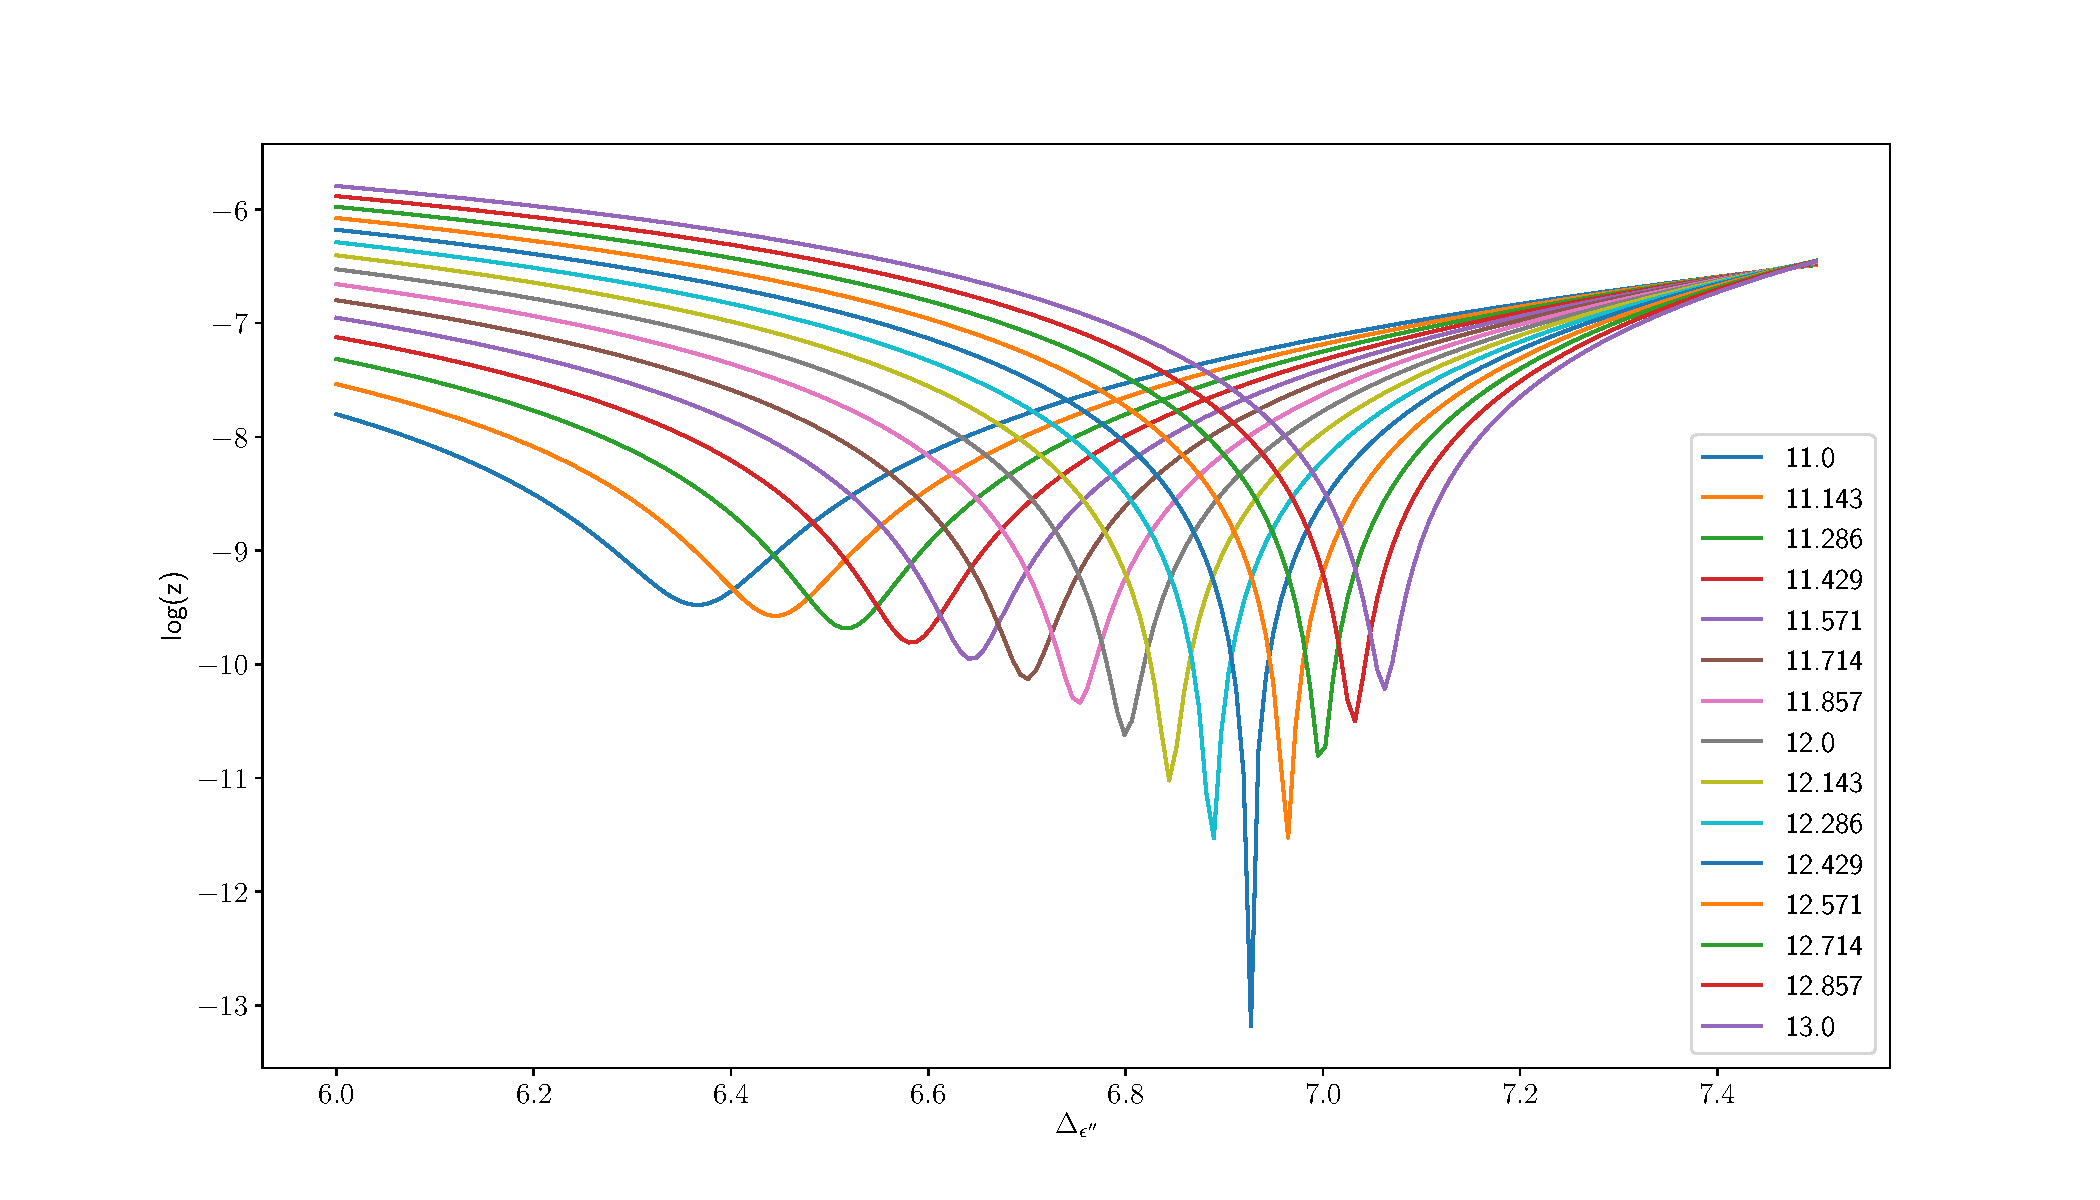
\includegraphics[scale=0.45]{Normal_N3_new.pdf}
    \caption{$N = 3$}
\end{subfigure}


\caption{Log of minimum singular value of the derivative matrix for different values of $\Delta_{\epsilon'''}$ for $N = 2$ and $N = 3$. A consistent solution is found when the minimum singular value is zero.}
\label{fig:res}
\end{figure}

Repeating the process for $N = 2$, we found the minimum singular value at
\begin{equation}
    \Delta_{\epsilon''} = 6.984, \hspace{0.5 in}\Delta_{\epsilon'''} = 12.4285
\end{equation}
with the OPE coefficients
\begin{center}
\begin{tabular}{L L L}
    a_{\epsilon}\lambda_{\phi\phi\epsilon} = 3.99, &a_{\epsilon'}\lambda_{\phi\phi\epsilon} = 1.359, &a_{\epsilon''}\lambda_{\phi\phi\epsilon''} = 0.143, \\
    a_{\epsilon'''}\lambda_{\phi\phi\epsilon'''} = 0.004,
    &a_{\sigma}^2 = 8.568,
    &\mu_{\sigma D}^2 = 0.07(26),\\
    \mu_{\phi\phi}^2 = 0.23(94).
\end{tabular}  
\end{center}
The search for the solution is plotted in Figure~\ref{fig:res}. Similarly, for $N = 3$, we found a consistent solution at
\begin{equation}
    \Delta_{\epsilon''} = 6.927, \hspace{0.5 in}\Delta_{\epsilon'''} = 12.4285
\end{equation}
with the OPE coefficients
\begin{center}
\begin{tabular}{L L L}
    a_{\epsilon}\lambda_{\phi\phi\epsilon} = 2.938, &a_{\epsilon'}\lambda_{\phi\phi\epsilon} = 1.026, &a_{\epsilon''}\lambda_{\phi\phi\epsilon''} = 0.118, \\
    a_{\epsilon'''}\lambda_{\phi\phi\epsilon'''} = 0.004,
    &a_{\sigma}^2 = 10.075,
    &\mu_{\sigma D}^2 = 0.0743,\\
    \mu_{\phi\phi}^2 = 0.2539.
\end{tabular}  
\end{center}
Notice that the dimensions $\Delta_{\epsilon''}$ and $\Delta_{\epsilon'''}$ are essentially the same as those for $N = 2$. However, the other CFT data is different. These are two different CFTs, but they have the same operators in their low-lying spectrum which is curious (maybe an artefact of the coarse grid?).

Finally, for $N = 4$, we have
\begin{equation}
    \Delta_{\epsilon''} = 6.897, \hspace{0.5 in}\Delta_{\epsilon'''} = 12.464
\end{equation}
with the OPE coefficients
\begin{center}
\begin{tabular}{L L L}
    a_{\epsilon}\lambda_{\phi\phi\epsilon} = 2.49, &a_{\epsilon'}\lambda_{\phi\phi\epsilon} = 0.883, &a_{\epsilon''}\lambda_{\phi\phi\epsilon''} = 0.107, \\
    a_{\epsilon'''}\lambda_{\phi\phi\epsilon'''} = 0.003,
    &a_{\sigma}^2 = 11.8823,
    &\mu_{\sigma D}^2 = 0.07643,\\
    \mu_{\phi\phi}^2 = 0.25696.
\end{tabular}  
\end{center}
\subsection{Comparison to large-$N$ results}
We compare our values of $a_\sigma$ and $\mu_{\phi\phi}$ to the large-$N$ results from \cite{Max}. The results are presented in Figure \ref{fig:compare}. 
\begin{figure}[H]
% \captionsetup[subfigure]{justification=centering}

\begin{subfigure}{\columnwidth}
    \centering
    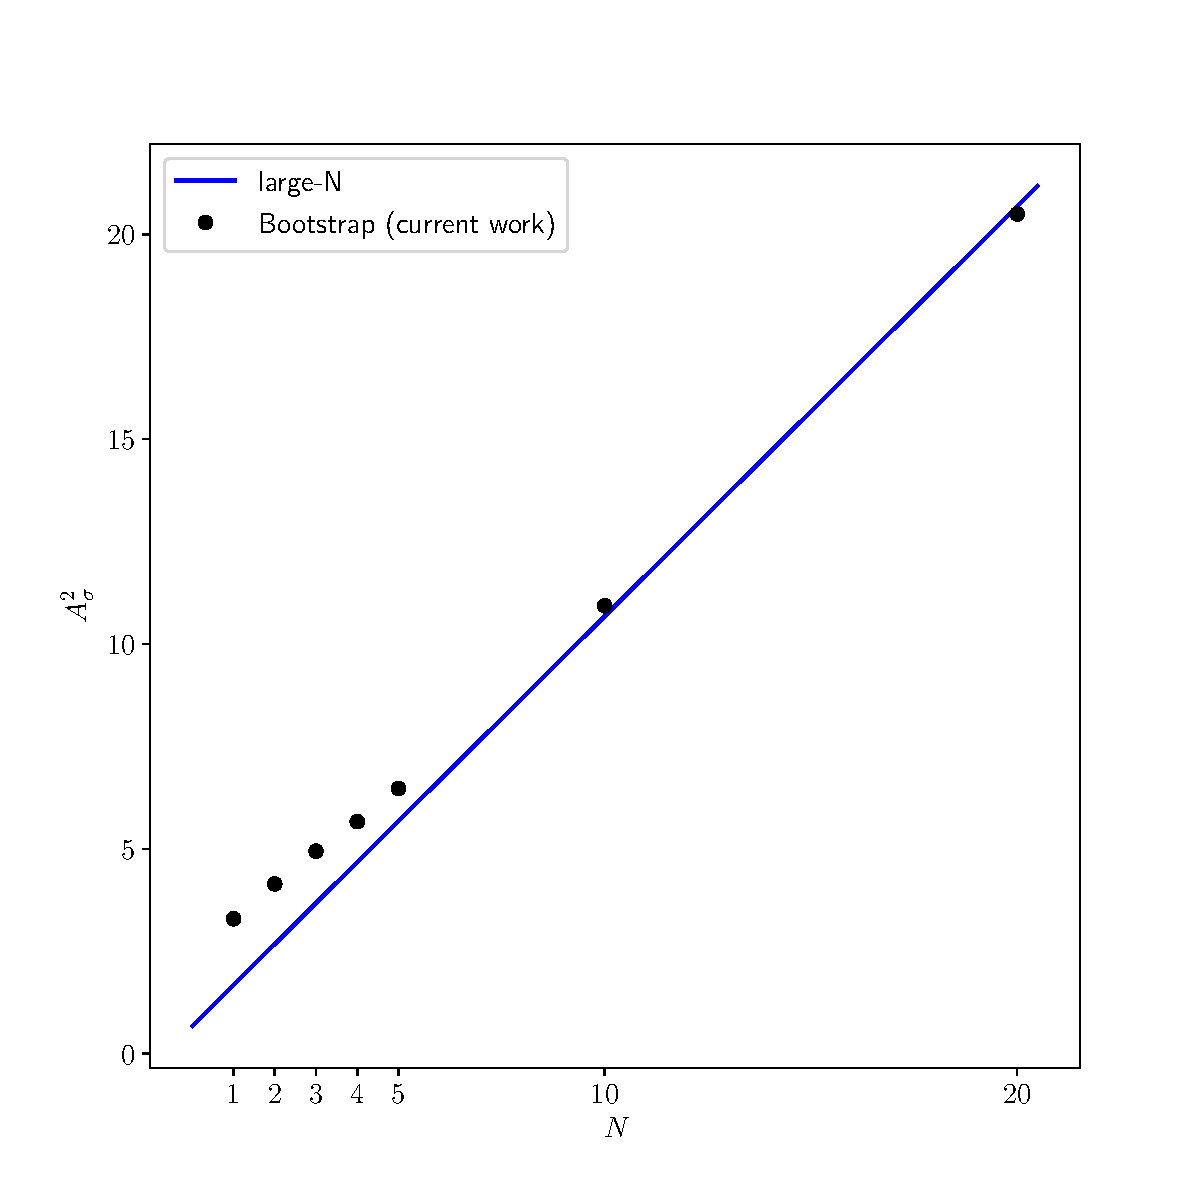
\includegraphics[scale=0.5]{AsigmaCompare.pdf}
\end{subfigure}
~

\begin{subfigure}{\columnwidth}
    \centering
    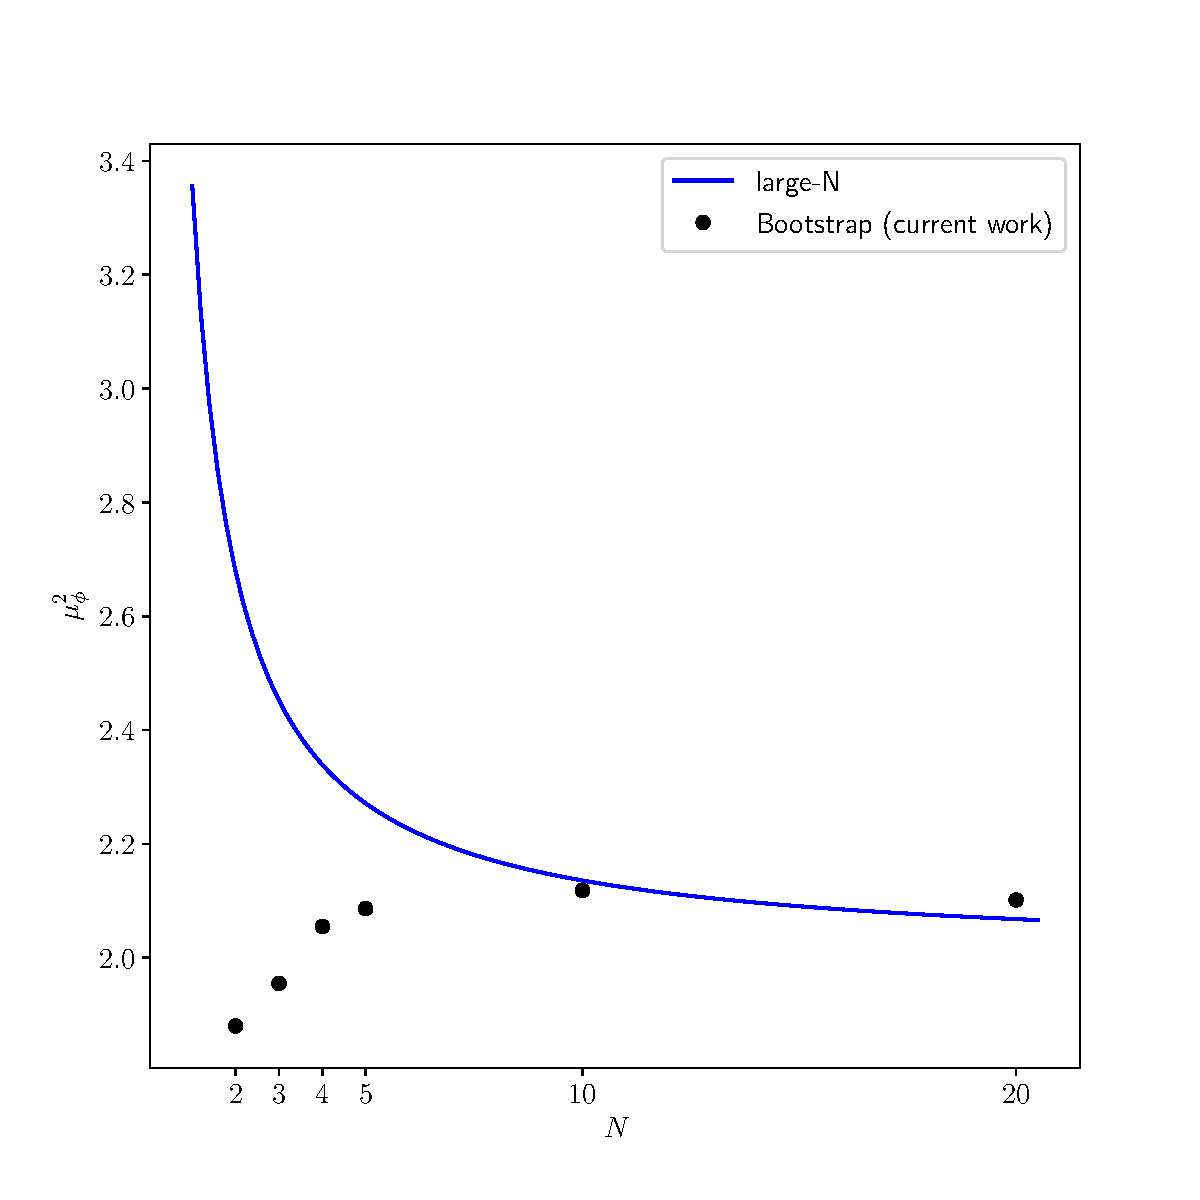
\includegraphics[scale=0.5]{muphi_compare.pdf}
\end{subfigure}

\caption{Bootstrap vs large-$N$: The plots compare results from \cite{Max} and our work. Dots represent bootstrap results. The OPE coefficients $A_{\sigma}$ and $\mu_\phi$ calculated in \cite{Max} differs from our $a_{\sigma}$ and $\mu_{\phi\phi}$ by a factor of $2^{\Delta_{\phi}}$ and $2^{\Delta_{\phi}-(d-1)}$ respectively; we plot here the rescaled values and NOT our bare results presented in Section \ref{sec:res} }
\label{fig:compare}
\end{figure}




% The amsmath package has many features. For example, you can use use
% \texttt{subequations} environment:
% \begin{subequations}\label{eq:y}
% \begin{align}
% \label{eq:y:1}
% a & = 1
% \\
% \label{eq:y:2}
% b & = 2
% \end{align}
% and it will continue to operate across the text also.
% \begin{equation}
% \label{eq:y:3}
% c = 3
% \end{equation}
% \end{subequations}
% The references will work as you'd expect: \eqref{eq:y:1},
% \eqref{eq:y:2} and \eqref{eq:y:3} are all part of \eqref{eq:y}.

% A similar solution is available for figures via the \texttt{subfigure}
% package (not loaded by default and not shown here). 
% All figures and tables should be referenced in the text and should be
% placed at the top of the page where they are first cited or in
% subsequent pages. Positioning them in the source file
% after the paragraph where you first reference them usually yield good
% results. See figure~\ref{fig:i} and table~\ref{tab:i}.

% \begin{figure}[tbp]
% \centering % \begin{center}/\end{center} takes some additional vertical space
% 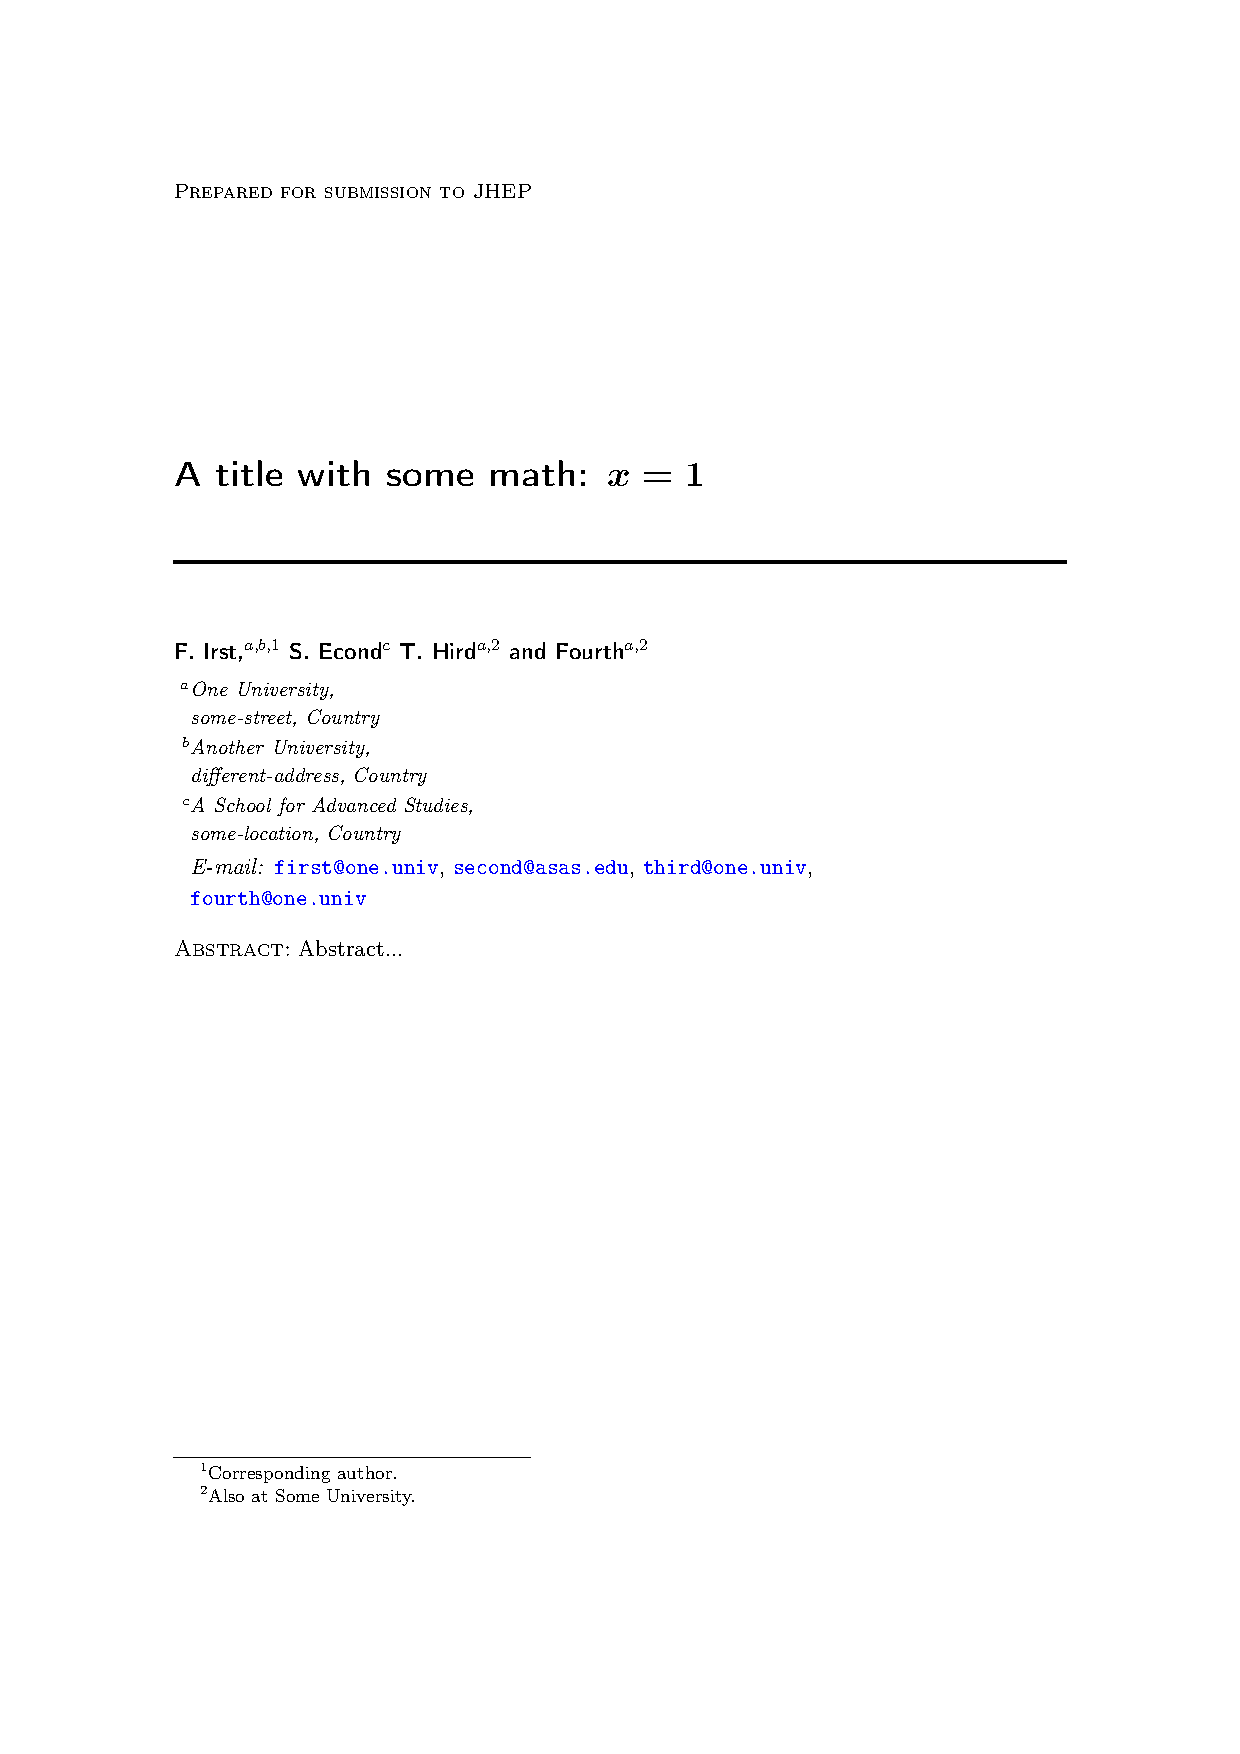
\includegraphics[width=.45\textwidth,trim=0 380 0 200,clip]{img1.pdf}
% \hfill
% 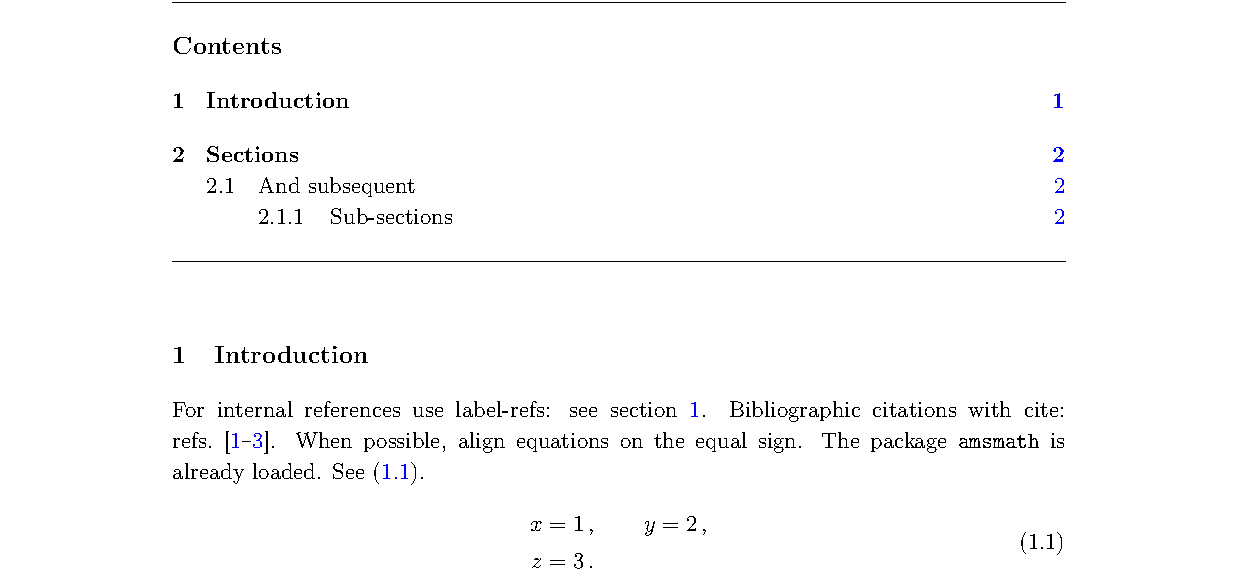
\includegraphics[width=.45\textwidth,origin=c,angle=180]{img2.pdf}
% % "\includegraphics" is very powerful; the graphicx package is already loaded
% \caption{\label{fig:i} Always give a caption.}
% \end{figure}

% \begin{table}[tbp]
% \centering
% \begin{tabular}{|lr|c|}
% \hline
% x&y&x and y\\
% \hline 
% a & b & a and b\\
% 1 & 2 & 1 and 2\\
% $\alpha$ & $\beta$ & $\alpha$ and $\beta$\\
% \hline
% \end{tabular}
% \caption{\label{tab:i} We prefer to have borders around the tables.}
% \end{table}

% We discourage the use of inline figures (wrapfigure), as they may be
% difficult to position if the page layout changes.

% We suggest not to abbreviate: ``section'', ``appendix'', ``figure''
% and ``table'', but ``eq.'' and ``ref.'' are welcome. Also, please do
% not use \texttt{\textbackslash emph} or \texttt{\textbackslash it} for
% latin abbreviaitons: i.e., et al., e.g., vs., etc.



% \section{Sections}
% \subsection{And subsequent}
% \subsubsection{Sub-sections}
% \paragraph{Up to paragraphs.} We find that having more levels usually
% reduces the clarity of the article. Also, we strongly discourage the
% use of non-numbered sections (e.g.~\texttt{\textbackslash
%   subsubsection*}).  Please also see the use of
% ``\texttt{\textbackslash texorpdfstring\{\}\{\}}'' to avoid warnings
% from the hyperref package when you have math in the section titles



% \appendix
% \section{Some title}
% Please always give a title also for appendices.





% \acknowledgments

% This is the most common positions for acknowledgments. A macro is
% available to maintain the same layout and spelling of the heading.

% \paragraph{Note added.} This is also a good position for notes added
% after the paper has been written.





% The bibliography will probably be heavily edited during typesetting.
% We'll parse it and, using the arxiv number or the journal data, will
% query inspire, trying to verify the data (this will probalby spot
% eventual typos) and retrive the document DOI and eventual errata.
% We however suggest to always provide author, title and journal data:
% in short all the informations that clearly identify a document.

\begin{thebibliography}{99}


\bibitem{Max}
Max A. Metlitski,
\emph{Boundary criticality of the O(N) model in d = 3 critically revisited},
\href{https://arxiv.org/abs/2009.05119}{arXiv:2009.05119} (2020)

\bibitem{Liendo}
P. Liendo, L. Rastelli and Balt C. van Rees,
\emph{The bootstrap program for boundary $CFT_d$}, JHEP, \href{https://link.springer.com/article/10.1007/JHEP07(2013)113}{07 (2013) 113}

\bibitem{Mcavity}
McAvity, D.M., and H. Osborn. \emph{Conformal Field Theories Near a Boundary in General Dimensions.} Nuclear Physics B 455.3 (1995): 522–576. \url{https://doi.org/10.1016/0550-3213(95)00476-9}

\bibitem{Gliozzi}
F. Gliozzi, P. Liendo, M. Meineri and A. Rago, \emph{Boundary and interface CFTs from the conformal bootstrap}, JHEP, \href{https://link.springer.com/article/10.1007/JHEP05(2015)036}{05 (2015) 036}

\bibitem{Kos}
F. Kos, D. Poland and D. Simmons-Duffin, \emph{Bootstraping the $O(N)$ vector models}, JHEP, \href{https://doi.org/10.1007/JHEP06(2014)091}{ 06 (2014) 091}

\bibitem{Leclair}
A. LeClair and J. Squires, \emph{Conformal bootstrap for percolation and polymers}, J. Stat. Mech. \url{https://doi.org/10.1088/1742-5468/aaf10a}

\bibitem{Guida}
R. Guida and J. Zinn-Justin, \emph{Critical exponents of the $N$-vector model}, J.Phys.A \href{https://iopscience.iop.org/article/10.1088/0305-4470/31/40/006}{31:8103-8121,1998} 



% Please avoid comments such as "For a review'', "For some examples",
% "and references therein" or move them in the text. In general,
% please leave only references in the bibliography and move all
% accessory text in footnotes.

% Also, please have only one work for each \bibitem.


\end{thebibliography}
\end{document}
